\documentclass[a4paper,12pt,onecolumn]{article}
\usepackage[utf8]{inputenc}
\usepackage{amsthm,amsmath,amscd}
\usepackage{pgfplots}
\pgfplotsset{compat=1.15}
\usetikzlibrary{arrows}
\usepackage{tikz-cd}
\tikzcdset{every label/.append style = {font = \small}}
\usepackage{xcolor}

\begin{document}

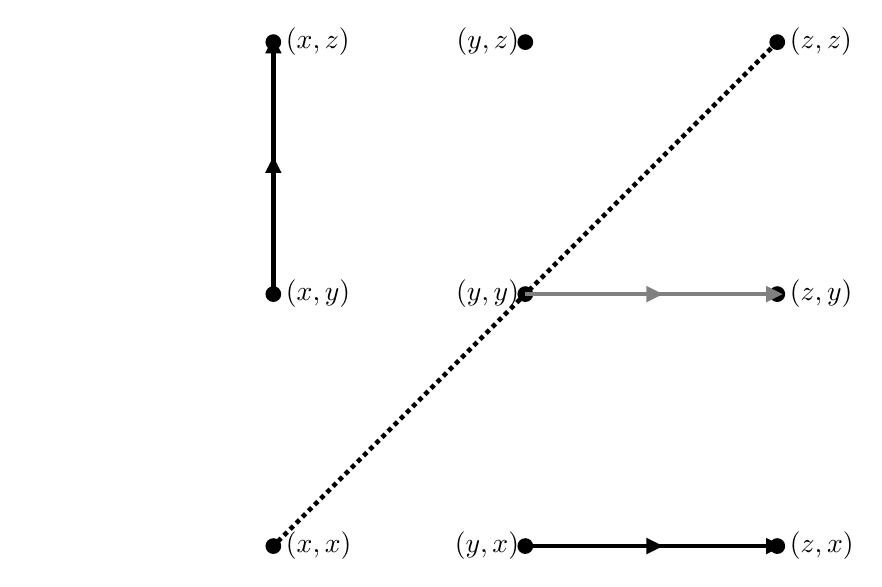
\begin{tikzpicture}[x=.8mm, y=.8mm, inner xsep=0pt, inner ysep=0pt, outer xsep=0pt, outer ysep=0pt]
		\definecolor{F}{rgb}{0,0,0}
		\path[fill=F] (30.00,110.00) circle (1.00mm);
		\path[fill=F] (30.00,70.00) circle (1.00mm);
		\path[fill=F] (70.00,110.00) circle (1.00mm);
		\path[fill=F] (70.00,70.00) circle (1.00mm);
		\path[fill=F] (30.00,30.00) circle (1.00mm);
		\path[fill=F] (70.00,30.00) circle (1.00mm);
		\path[fill=F] (110.00,110.00) circle (1.00mm);
		\path[fill=F] (110.00,70.00) circle (1.00mm);
		\path[fill=F] (110.00,30.00) circle (1.00mm);
		\definecolor{T}{rgb}{0,0,0}
		\draw[T] (32.00,69.00) node[anchor=base west]{ {$(x,y)$}};
		\draw[T] (32.00,109.00) node[anchor=base west]{ {$(x,z)$}};
		\draw[T] (69.00,109.00) node[anchor=base east]{ {$(y,z)$}};
		\draw[T] (112.00,109.00) node[anchor=base west]{ {$(z,z)$}};
		\draw[T] (112.00,69.00) node[anchor=base west]{ {$(z,y)$}};
		\draw[T] (112.00,29.00) node[anchor=base west]{ {$(z,x)$}};
		\draw[T] (69.00,29.00) node[anchor=base east]{ {$(y,x)$}};
		\draw[T] (32.00,29.00) node[anchor=base west]{ {$(x,x)$}};
		\draw[T] (69.00,69.00) node[anchor=base east]{ {$(y,y)$}};
		\path[] (5.00,107.00) -- (-9.00,76.00);
		\definecolor{L}{rgb}{0,0,0}
		\path[line width=0.60mm, draw=L, dash pattern=on 0.60mm off 0.50mm] (110.00,110.00) -- (30.00,30.00);
		\definecolor{L}{rgb}{0.502,0.502,0.502}
		\path[line width=0.60mm, draw=L] (110.00,70.00) -- (70.00,70.00);
		\definecolor{F}{rgb}{0.502,0.502,0.502}
		\path[line width=0.60mm, draw=L, fill=F] (110.00,70.00) -- (108.60,70.70) -- (108.60,69.30) -- (110.00,70.00) -- cycle;
		\path[line width=0.60mm, draw=L] (91.00,70.00) -- (70.00,70.00);
		\path[line width=0.60mm, draw=L, fill=F] (91.00,70.00) -- (89.60,70.70) -- (89.60,69.30) -- (91.00,70.00) -- cycle;
		\definecolor{L}{rgb}{0,0,0}
		\path[line width=0.60mm, draw=L] (91.00,30.00) -- (70.00,30.00);
		\definecolor{F}{rgb}{0,0,0}
		\path[line width=0.60mm, draw=L, fill=F] (91.00,30.00) -- (89.60,30.70) -- (89.60,29.30) -- (91.00,30.00) -- cycle;
		\path[line width=0.60mm, draw=L] (110.00,30.00) -- (70.00,30.00);
		\path[line width=0.60mm, draw=L, fill=F] (110.00,30.00) -- (108.60,30.70) -- (108.60,29.30) -- (110.00,30.00) -- cycle;
		\path[line width=0.60mm, draw=L] (30.00,91.00) -- (30.00,70.00);
		\path[line width=0.60mm, draw=L, fill=F] (30.00,91.00) -- (29.30,89.60) -- (30.70,89.60) -- (30.00,91.00) -- cycle;
		\path[line width=0.60mm, draw=L] (30.00,110.00) -- (30.00,70.00);
		\path[line width=0.60mm, draw=L, fill=F] (30.00,110.00) -- (29.30,108.60) -- (30.70,108.60) -- (30.00,110.00) -- cycle;
	\end{tikzpicture}

\end{document}